\section{Introduction}
Robots must be able to understand natural language if they are to efficiently collaborate with humans.
In order to achieve this goal, the problem of associating phrase with real-world objects and actions, commonly referred to as the grounding problem, has emerged as a focus of new research in robotics (cite G3,DCG, etc.).\\
\indent While traditional solutions to the grounding problem may be trained to ground a fixed set of phrases to a fixed set objects, such methods fail to reason intelligently about unknown phrases or objects that have never been encountered in training.
Furthermore, current techniques often assume that the location of the object being grounded to is known (e.g. phrases refer to objects that are currently perceived or localized within a known map).
As a result, a robot will pick the most likely perceived grounding rather than exploring its surroundings.\\
\indent To assume that language will be drawn from a fixed set and to assume that language only refers to known, perceived objects is unsafe in the real world.
Humans regularly draw upon context-specific lexicons that the general population does not recognize; however, training a robot to know every possible meaning of every possible word is infeasible and inefficient.
At the same time, humans often refer to objects whose locations are fundamentally unknown.
Attempting to reason over the space of all possible maps, however, is similarly computationally infeasible.\\
\indent Na{\"i}ve solutions to these problems 
\begin{figure}[t]
	\centering
	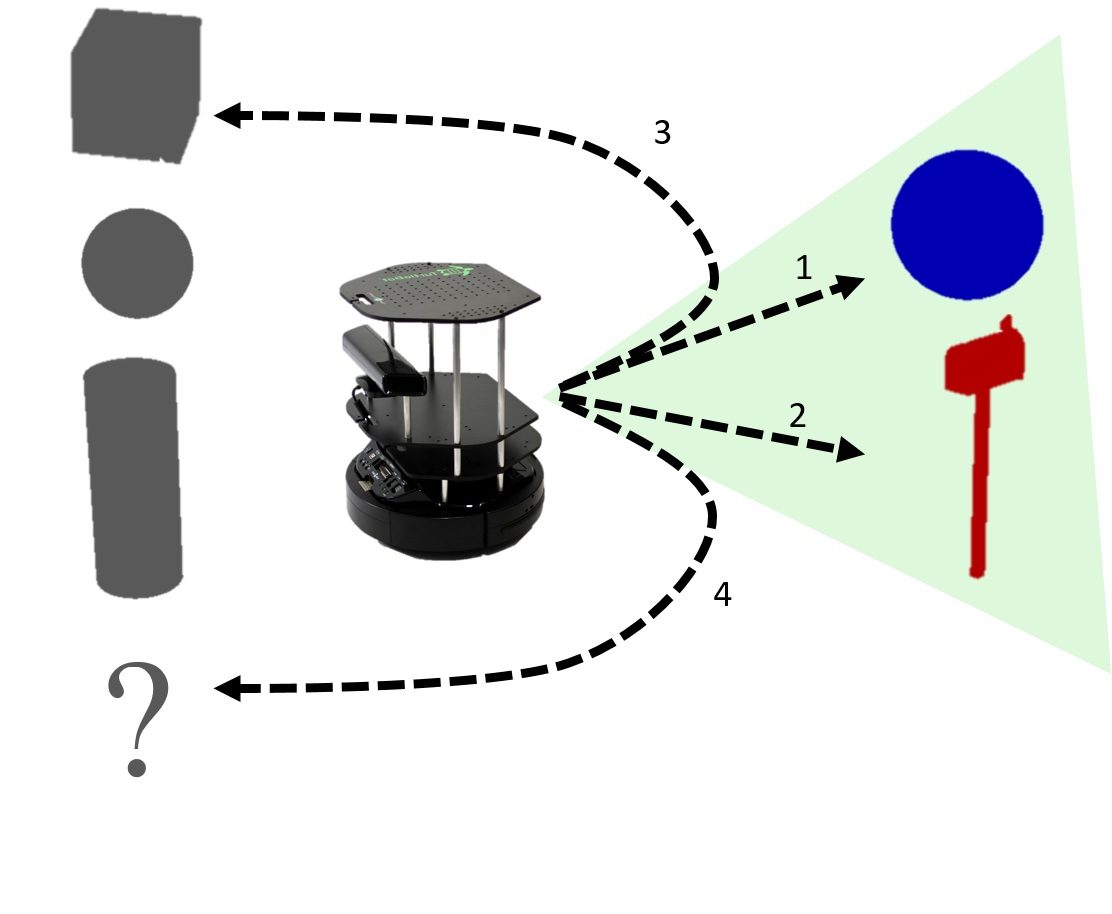
\includegraphics[width=8.5cm]{intro_pic}
	\caption{In this example, DCG-UPUP-Away has been trained only with cubes, spheres, and cylinders. DCG-UPUP-Away may ground phrases to known perceived objects (1), unknown perceived objects (2), known hypothesized objects (3), or unknown hypothetical objects (4).}
	\label{fig:intro_pic}
\end{figure}